% The following answers were used to create this image:
% - http://tex.stackexchange.com/a/373/5645 - Torus
\documentclass[border=2pt]{standalone}
\usepackage{amsmath,amssymb}
\usepackage{tikz}
\usetikzlibrary{patterns,arrows,positioning}

\begin{document}
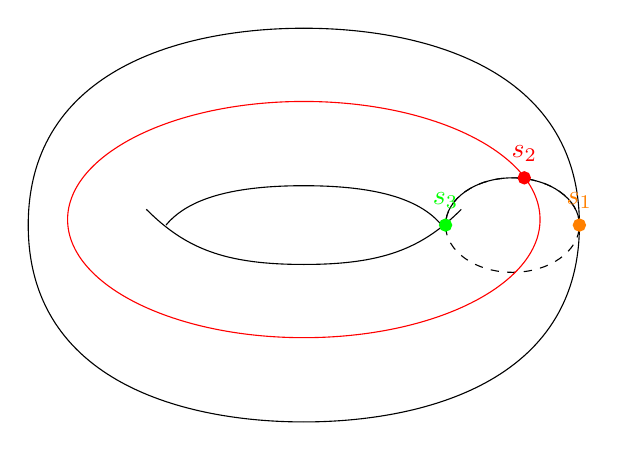
\begin{tikzpicture}
\tikzstyle{point}=[circle,thick,draw=black,fill=black,inner sep=0pt,minimum width=4pt,minimum height=4pt]
\draw (-3.5,0) .. controls (-3.5,2) and (-1.5,2.5) .. (0,2.5);
\draw[xscale=-1] (-3.5,0) .. controls (-3.5,2) and (-1.5,2.5) .. (0,2.5);
\draw[rotate=180] (-3.5,0) .. controls (-3.5,2) and (-1.5,2.5) .. (0,2.5);
\draw[yscale=-1] (-3.5,0) .. controls (-3.5,2) and (-1.5,2.5) .. (0,2.5);

\draw (-2,.2) .. controls (-1.5,-0.3) and (-1,-0.5) .. (0,-.5) .. controls (1,-0.5) and (1.5,-0.3) .. (2,0.2);
\draw (-1.75,0) .. controls (-1.5,0.3) and (-1,0.5) .. (0,.5) .. controls (1,0.5) and (1.5,0.3) .. (1.75,0);

\draw[dashed] (2.65,0) ellipse (0.85 and 0.6);
\draw (3.5,0) arc (-360:-180:0.85 and 0.6);

\node (s1)[point,orange,label={[label distance=0mm]\color{orange}$s_1$}] at (3.5,0) {};
\node (s2)[point,red,label={[label distance=0mm]\color{red}$s_2$}] at (2.8,0.6) {};
\node (s3)[point,green,label={[label distance=0mm]\color{green}$s_3$}] at (1.8,0) {};
\draw[red] (0,0.07) ellipse (3cm and 1.5cm);
\end{tikzpicture}
\end{document}
